%%This is a very basic article template.
%%There is just one section and two subsections.
%\documentclass[12pt,oneside,a4paper,doublespacing]{article} % for submission
\documentclass[11pt,oneside]{article} % for sharing


\usepackage{appendix}
\usepackage{amsmath}
\usepackage{caption}
\usepackage{placeins}
\usepackage{graphicx}
\usepackage{subcaption}
\usepackage{longtable}
\usepackage{setspace}
%\usepackage{tikz}
\usepackage{booktabs}
\usepackage{xcolor,colortbl}
\usepackage{chngpage}
%\usepackage[active,tightpage]{preview}
\usepackage{natbib}
\bibpunct{(}{)}{,}{a}{}{;} 
\usepackage{url}
\usepackage{nth}
\usepackage{authblk}
%\usepackage{pdfsync}

\renewcommand{\listtablename}{List of Appendix Tables}
\newcolumntype{C}[1]{>{\centering\let\newline\\\arraybackslash\hspace{0pt}}m{#1}}
\newcolumntype{L}[1]{>{\raggedright\let\newline\\\arraybackslash\hspace{0pt}}m{#1}}

% working on this need to concatenate file name based on sex and variable name
%\newcommand\Cell[1]{{\raisebox{-0.05in}{\includegraphics[height=.2in,width=.2in]{Figures/ColorCodes/\expandafter#1}}}}  

\newcommand\ackn[1]{%
  \begingroup
  \renewcommand\thefootnote{}\footnote{#1}%
  \addtocounter{footnote}{-1}%
  \endgroup
}

\defcitealias{HMD}{HMD}


\begin{document}

\title{A unified model of demographic time}

\author[1]{Tim Riffe\thanks{triffe@demog.berkeley.edu}}
\author[2]{Jonas Sch{\"o}ley}
\author[2]{Francisco Villavicencio}
\affil[1]{Max Planck Institute for Demographic Research}
\affil[2]{University of Southern Denmark}

%\author{[Authors]}


\maketitle

\begin{abstract}
We describe a three-dimensional model that relates six different aspects of
lifespans and time. The six aspects of demographic time considered are
chronological age, thanatological age, lifespan, year of birth, year of death,
and period. Two versions of the model are described: a relatively intuitive
extension of the right-angled Lexis diagram, and an isotropic extension based on
the regular tetrahedron. \ackn{The work reported in this manuscript was begun by
the first author while at the Department of Demography at the University of
California, Berkeley, and was supported by the U.S.
National Institute On Aging of the National Institutes of Health under award
numbers R01-AG011552 and R01-AG040245. The content is solely the responsibility of the authors and does not necessarily represent the official views of the funding agencies.}

\end{abstract}


The so-called Lexis diagram relates the chronological age (A), period (P), and
birth cohort (C) indices of demographic time, APC, but it does not account
for remaining years of life (thanatological age), and other related time
indices.
The thanatological counterpart to APC is an identity between thanatological age (T), period (P), and death cohort (D), TPD. A third identity exists between
chronological age (A), thanatological age (T), and lifespan (L), ATL, and a
fourth between year of birth (C), year of death (D) and lifespan (L), CDL.
Each of these four tripartite identities may be sufficiently described by any
two of its consituent indices, making the third index redundant. Each of these
four identities also lacks a major dimension of time. The ATL identity lacks
calendar time, the CDL identity is ageless, APC lacks years left, and TPD lacks years lived. 

To my knowledge, the only tripartite identity that has received serious
treatment at this point in time is the APC identity. Different aspects of the
APC identity have been discussed since at least 1868
\citep{knapp1868ermittlung}, and discussion remains lively at the time of this
writing. Here it is our objective to relate the six major indices of time to a
geometric identity, in much the same spirit as the work on APC done
between the late 1860s and mid 1880s.\footnote{See e.g., \citet{keiding2011age}
for an overview of that literature.} 

Each of the four tripartite identities may be thought of as a
two-dimensional plane fully defined by any two of its three constituent time
indices.
In this case, we may imagine the third ``lacking'' dimension as spatial for the sake of conceptualization.
Having a third dimension implies a multitude of parallel planes for the given identity, each plane
belonging to a unique value of the third time dimension. Any of the
identities can be extended in this way to fill a space. A space derived by
extending any of the tripartite identies into its lacking dimension implies each of the
other tripartite identities, making a total of six time indices. In essence, the
four tripartite identities may be thought of as parallel to the four faces of a
tetrahedron. In this case, the four ``lacking'' dimensions may be assigned to
the four vertices of the tetrahedron, and the six demographic time indices match
to the six edges of the tetrahedron. It is this three-dimensional construct that
unifies the six indices of demographic time, and which I decribe in this
paper.

we have mentioned six different aspects of demographic time. Other combinations
of three of these are possible, but they automatically imply the above-mentioned
three-dimensionalization. In imagining this three-dimensional relationship,
it may help to first consider its extension. Some indices are limited
by our maximum length of life, $\omega$, while others are boundless. A, T, and L are clearly in the range $[0,\omega]$. P, C, and D are bounded only by the inception and extinction of our species, but may be
thought of as boundless for practicality, or by our earliest and most recent
observations for even more practicality. As an abstraction, however, the
dimension of calendar time in this model is infinite. Of the four identities,
only one lacks an unbounded dimension, the ATL. Adding the absent dimension to
ATL therefore makes it boundless. In this way, we may imagine a prism-like
construct, where A, T, and L, compose the faces of a triangular
cross-section of said prism, which extends infinitely ``through'' the triangle.
We can think of the ATL triangle passing through time, extending the population
forward to infinity. In this case, the ATL triangle may take either the period
or cohort perspectives, and this will be explained later. 

There are also
numerous ways that this three dimensional construct can be proportioned, of
which I present two in this paper. The first stems from the respect given to right angles in the most
common representation of the Lexis diagram. For this reason, it will likely be
the most intuitive rendition of the model, and it will be presented first. The
second version presented is isotropic with respect to time units in each of the
six temporal indices. In this case, the four tripartite identities are based on
equilateral triangles between their three constituent indices, and the four
planes are joined together such that each is parallel to a face from the regular
tetrahedron, a construct known in geometry as an octahedral-tetrahedral
honeycomb.

In this paper we first state the relationships between all six dimensions of
demographic time. The APC, TDL, and ATL planes are introduced as degenerate
cases of the unified model. The case of the ATLC cross-sectional plane is
introduced, followed by the full three-dimensional unified model, the APCTDL
model.
Finally, we demonstrate the use of this coordinate system for the case of
end-of-life trajectories of some characteristics of morbidity. I explain the
utility of this model by demonstrating a case where heterogeneity with respect
to unaccounted-for time dimensions has caused serious misunderstandings in the
scientific literature and in public policy.

\section*{Intersecting planes}

The  model can be introduced in terms of four planes intersecting in
Euclidean 3d space. Two of the planes motivate the model, and the other two
are in this case artifactual, although they may have demographic meaning. The
first plane is the widely used APC plane. This plane omits remaining years of
life (T). 

\subsection*{APC}
The Lexis diagram has long been used in demography to relate chronological age
(A) with birth cohorts (C) and calendar years (P). Since the so-called Lexis
diagram could have been named for others
\citep{vandeschrick2001lexis,keiding2011age}, and since we compare with other
temporal configurations, let us refer to it as the APC diagram, as seen in
Figure~\ref{APCright}
When a value (data) is structured by APC coordinates, we refer to it as an APC surface.

\begin{figure}[b!]
    \centering
    % figure made in R/LexisStandard.R
    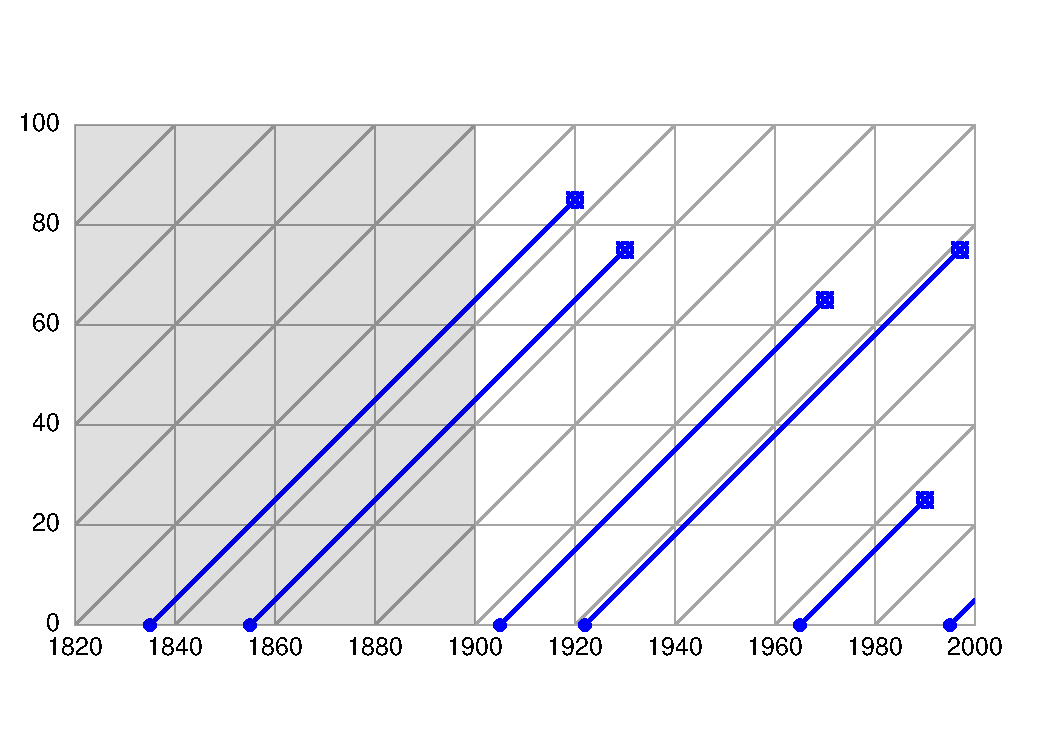
\includegraphics[scale=.7]{Figures/LabPres/APC2.pdf}
    \caption{Lifelines in the APC diagram}
    \label{APCright}
\end{figure} 

The APC diagram in Figure~\ref{APCright} represents years lived on the y axis,
calendar years on the x axis, and birth cohorts as the right-ascending
diagonals. This is the most common of several possible configurations
of the APC dimensions. Individual lifelines are aligned in the cohort direction,
starting with birth (filled circle) at chronological age zero, and death ()

Any APC surface can be interpreted along each of these
three dimensions of temporal structure. Such interpretation is a descriptive
task, and it does not succumb to problems of overidentification. Variation along
these three dimensions can not be parsimonsiously separated into the three
effects of A, P, and C. This is the so-called APC problem, and it is not the concern of the
present work. 

It has long been noted \citep{zeuner1869abhandlungen, perozzo1880della} that the
birth cohort dimension, as represented in Figure~\ref{APCright}, is relatively
longer than either the age or years axes. If a right angle and unity aspect
ratio is forced between any two of the APC dimensions, the third dimension is always be
stretched by $\sqrt{2}$. Another long-standing, but less common variant, is to
represent

\FloatBarrier

\subsection*{TPD}

Thanatological age (T), period (P) and death cohort (D) form a coordinate system
best imagined as the opposite of APC. One may take the same lifelines from
Figure~\ref{APCright} and realign them in descending fashion to create the
diagram in Figure~\ref{TPDright}

\begin{figure}[b!]
    \centering
    % figure made in R/LexisStandard.R
    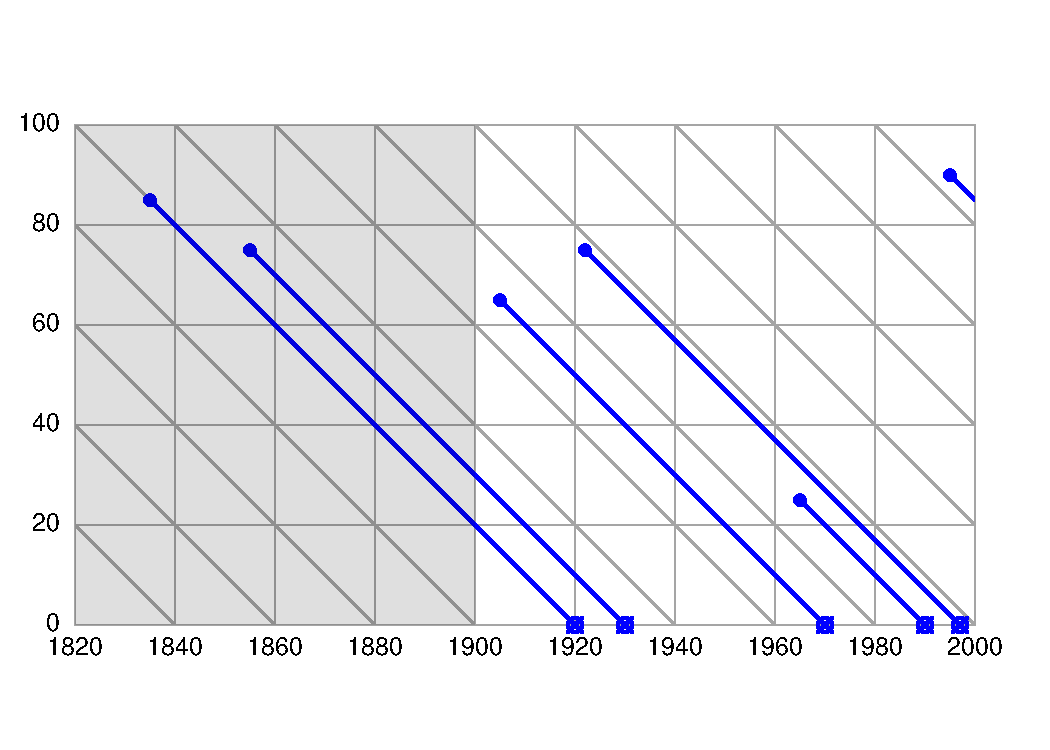
\includegraphics[scale=.7]{Figures/LabPres/TPD2.pdf}
    \caption{Lifelines in the TPD diagram}
    \label{TPDright}
\end{figure} 

\subsection*{ATL}
The second plane is ATL, a valid coordinate system for
processes that vary over the lifecourse, but not over time (P). Since the
lifecourse belongs to the cohort perspective, it is best to think of the ATL
plane as belonging to some particular birth cohort. Alternatively, an ATL
triangle may be taken as a cross-section along through the period dimension, a
sort of synthetic ATL plane.



\section*{APCT}
I propose a geometric
identity that unifies all such temporal notions into a single (simple) spatial
relationship that serves as an omnibus conceptual aid to demographers, much as
the Lexis diagram does for APC relationships. The full result is a three
dimensional space that can be disected by any of four different planes,
each of which is parallel to the faces of a regular tetrahedron (see
Figure~\ref{fig:APCT} for a first mock-up of the model).
Each dissecting plane relates three indices of demographic time in proportion to one
another (1:1:1 ternary aspect ratio). The complete space can be described in
geometry nomenclature as the tetrahedral-octahedral honeycomb, which is a kind of space-filling tessellation.\footnote{Constructs following
this geometry exist both in nature and in man-made structures.} 
One of these planes is the familar Lexis plane (horizontal planes in
Figure~\ref{fig:APCT}, and the other three will be new surprises for
demographers. This three dimensional space is not only useful for the sake of formalizing observed temporal relationships, but also for encolosing
demographic time in the past and future (e.g., before the first census and after
the most recent census). 

\begin{figure}[!h]
\centering
\caption[cap]{A mock-up example of the unified model of demographic
time.\footnotemark}
\label{fig:APCT}
	\includegraphics[bb=0 0 3264 2448, width=\textwidth]{Figures/PhysicalModel.jpg}
\end{figure}
\footnotetext{This and other figures to be replaced with vector graphics, although
	I may bring this model to the presentation, since it helps explain concepts.}

A property of the geometry that I propose is that
the time units in every direction (with respect to each index) are proportional. The Lexis
diagram based on right angles and $45^\circ$ birth cohort lines does not have
this property, whereas Lexis diagrams and surfaces based on equilateral
triangles, such as some early proposals \citep[inter
alia, ][]{lexis1875einleitung, lewin1876rapport}, the masterful stereogram of
\citet{perozzo1880della}, or the more recent APC diagram
of \citet{ryder1980cohort}, do have this property. The disecting planes of the
model I propose are likewise composed of equilateral triangles. In Lexis
nomenclature, the 3d projections of an AP square, and AC or PC
parallelograms are all congruent shapes known as regular trigonal trapezohedra
(RTT). The orientation
of a given RTT uniquely defines the Lexis shape in question. Similar constructs
exist in the other time dimensions, and these will also be described. 


\bibliographystyle{plainnat}
  \bibliography{references} 



\end{document}